\chapter{ROOM Concepts}

This chapter gives an overview over the ROOM language elements and their textual and graphical notation.
The formal ROOM grammar based on Xtext (EBNF) you can find here: "ROOM Grammar":http://git.eclipse.org/c/etrice/org.eclipse.etrice.git/tree/plugins/org.eclipse.etrice.core.room/src/org/eclipse/etrice/core/Room.xtext

\section{Actors}

\subsection{Description}
 
The actor is the basic structural building block for building systems with ROOM. An actor can be refined hierarchically and thus can be of arbitrarily large scope. Ports define the interface of an actor. An Actor can also have a behavior usually defined by a finite state machine.

\subsection{Motivation}

\begin{itemize}
\item Actors enable the construction of hierarchical structures by composition and layering
\item Actors have their own logical thread of execution
\item Actors can be freely deployed
\item Actors define potentially reusable blocks
\end{itemize}

\subsection{Notation}


\begin{table}
\caption{Actor Class Notation}
\begin{tabular}{|l|l|l|}
\hline
 \textbf{Element} & \textbf{Graphical Notation} & \textbf{Textual Notation} \\ \hline
  ActorClass & 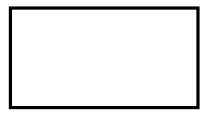
\includegraphics{images/040-ActorClassNotation.png} & 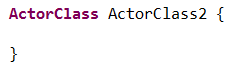
\includegraphics{images/040-ActorClassTextualNotation.png} \\ \hline
  ActorRef & 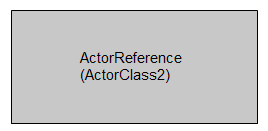
\includegraphics{images/040-ActorReferenceNotation.png} & 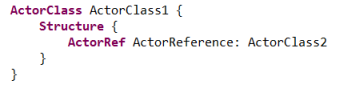
\includegraphics{images/040-ActorReferenceTextualNotation.png} \\ \hline
\end{tabular}
\end{table}

% <table title="Actor Class Notation" frame="box" border="2" cellpadding="3" cellspacing="0" >
	% <tr>
		% <td align="center">*Element*</td>
		% <td align="center">*Graphical Notation*</td>
		% <td align="center">*Textual Notation*</td>
	% </tr>
	% <tr>
		% <td>ActorClass</td>
		% <td>!images/040-ActorClassNotation.png!</td>
		% <td>!images/040-ActorClassTextualNotation.png!</td>
	% </tr>
	% <tr>
		% <td>ActorRef</td>
		% <td>!images/040-ActorReferenceNotation.png!</td>
		% <td>!images/040-ActorReferenceTextualNotation.png!</td>
	% </tr>
% </table> 


\subsection{Details}

\subsubsection{Actor Classes, Actor References, Ports and Bindings}

An \textbf{ActorClass} defines the type (or blueprint) of an actor. Hierarchies are built by ActorClasses that contain \textbf{ActorReferences} which have another ActorClass as type. The interface of an ActorClass is always defined by Ports. The ActorClass can also contain Attributes, Operations and a finite state machine. 

\textbf{External Ports} define the external interface of an actor and are defined in the *Interface* section of the ActorClass.

\textbf{Internal Ports} define the internal interface of an actor and are defined in the *Structure* section of the ActorClass.

\textbf{Bindings} connect Ports inside an ActorClass.

Example:

\begin{table}
\caption{Actor Class Example}
\begin{tabular}{|l|l|l|}
\hline
 \textbf{Graphical Notation} & \textbf{Textual Notation} \\ \hline
 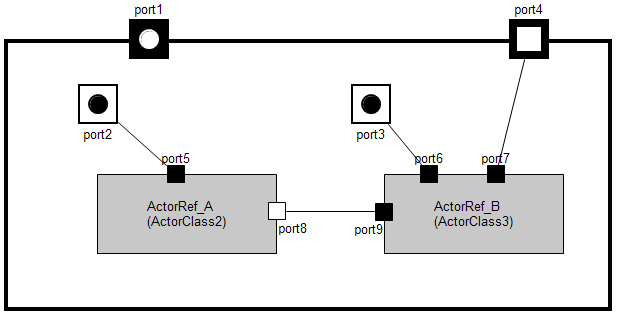
\includegraphics{images/040-ActorClass.png} & 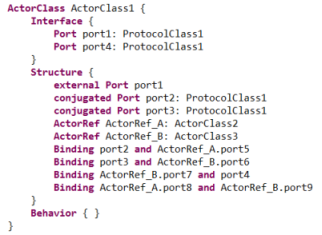
\includegraphics{images/040-ActorClassExampleTextualNotation.png} \\ \hline
 \end{tabular}
 \end{table}
 
% <table title="Actor Class Example" frame="box" border="2" cellpadding="3" cellspacing="0" >
	% <tr>
		% <td align="center">*Graphical Notation*</td>
		% <td align="center">*Textual Notation*</td>
	% </tr>
	% <tr>
		% <td>!images/040-ActorClass.png!</td>
		% <td>!images/040-ActorClassExampleTextualNotation.png!</td>
	% </tr>
% </table> 

\begin{itemize}
\item \textbf{ActorClass1} contains two ActorReferences (of ActorClass2 and ActorClass3)
\item \textit{port1} is a \textbf{External End Port}. Since it connects external Actors with the behavior of the ActorClass, it is defined in the \textbf{Interface} section and the \textbf{Structure} section of the ActorClass.
\item \textit{port2} and \textit{port3} are \textbf{Internal End Ports} and can only be connected to the ports of contained ActorReferences. Internal End Ports connect the Behavior of an ActorClass with its contained ActorReferences.
\item \textit{port4} is a relay port and connects external Actors to contained ActorReferences. This port can not be accessed by the behavior of the ActorClass.
\item \textit{port5} through \textit{port9} are Ports of contained ActorReferences. \textit{port8} and \textit{port9} can communicate without interference with the containing ActorClass.
\item \textbf{Bindings} can connect ports of the ActorClass and its contained ActorReferences. 
\end{itemize}

\subsubsection{Attributes}

Attributes are part of the Structure of an ActorClass. They can be of a PrimitiveType or a DataClass.

Example:

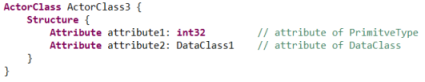
\includegraphics{images/040-ActorClassAttributes.png}
% !images/040-ActorClassAttributes.png!

\subsubsection{Operations}

Operations are part of the Behavior of an ActorClass.  Arguments and return values can be of a PrimitiveType or a DataClass. DataClasses can be passed by value (implicit) or by reference (keyword \textbf{ref}).

Example:

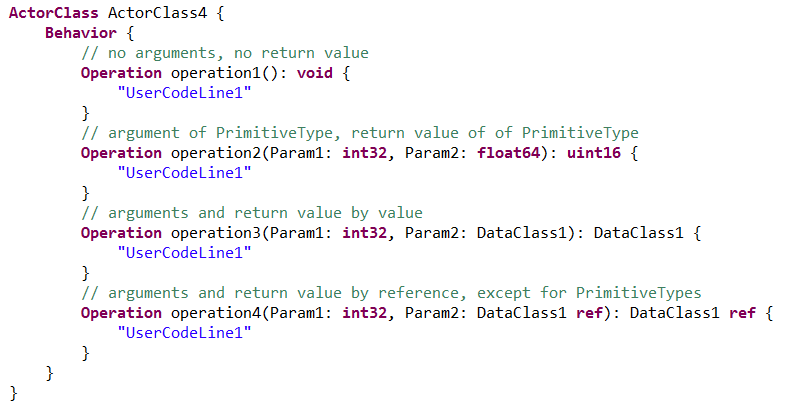
\includegraphics{images/040-ActorClassOperations.png}
% !images/040-ActorClassOperations.png!

\section{Protocols}

\subsection{Description}

A ProtocolClass defines a set of incoming and outgoing messages that can be exchanged between two ports.
The exact semantics of a message is defined by the execution model.

\subsection{Motivation}

\begin{itemize}
\item ProtocolClasses provide a reusable interface specification for ports
\item ProtocolClasses can optionally specify valid message exchange sequences
\end{itemize}

\subsection{Notation}

ProtocolClasses have only textual notation. 
The example defines a ProtocolClass with 2 incoming and two outgoing messages. Messages can have data attached. The data can be of a primitive type (e.g. int32, float64, ...) or a DataClass.

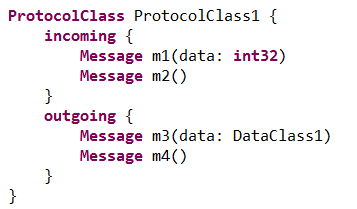
\includegraphics{images/040-ProtocolClassTextualNotation.png}
!images/040-ProtocolClassTextualNotation.png!

\section{Ports}

\subsection{Description}

Ports are the only interfaces of actors. A port has always a protocol assigned. 
Service Access Points (SAP) and Service Provision Points (SPP) are specialized ports that are used to define layering.

\subsection{Motivation}

\begin{itemize}
\item Ports decouple interface definition (Protocols) from interface usage
\item Ports decouple the logical interface from the transport 
\end{itemize}

\subsection{Notation}

\subsubsection{Class Ports}

These symbols can only appear on the border of an actor class symbol. 

Ports that define an external interface of the ActorClass, are defined in the \textit{Interface}. Ports that define an internal interface are defined in the \textit{Structure} (e.g. internal ports).
\begin{itemize}
\item \textbf{External End Ports} are defined in the Interface and the Structure
\item \textbf{Internal End Ports} are only defined in the Structure
\item \textbf{Relay Ports} are only defined in the Interface
\item \textbf{End Ports} are always connected to the internal behavior of the ActorClass
\item \textbf{Replicated Ports} can be defined with a fixed replication factor ( e.g. \textit{Port port18 [ 5 ]: ProtocolClass1} ) or a variable replication factor (e.g. \textit{Port port18[ * ]: ProtocolClass1} )
\end{itemize}

\begin{table}
\caption{Class Port Notation}
\begin{tabular}{|l|l|l|}
\hline
 \textbf{Element} & \textbf{Graphical Notation} & \textbf{Textual Notation} \\ \hline
 Class End Port & 
\includegraphics{images/040-ClassEndPort.png} & \\ \hline
 Class End Port & 
\includegraphics{images/040-ConjugatedClassEndPort.png} & \\ \hline
 Class Relay Port & 
\includegraphics{images/040-ClassRelayPort.png} & \\ \hline
 Conjugated Class Relay Port & 
\includegraphics{images/040-ConjugatedClassRelayPort.png} & \\ \hline
 Replicated Class End Port & 
\includegraphics{images/040-ReplicatedClassEndPort.png} & \\ \hline
 Conjugated Replicated Class End Port & 
\includegraphics{images/040-ConjugatedReplicatedClassEndPort.png} & \\ \hline
 Replicated Class Relay Port & 
\includegraphics{images/040-ReplicatedClassRelayPort.png} & \\ \hline
 Conjugated Replicated Class Relay Port & 
\includegraphics{images/040-ConjugatedReplicatedClassRelayPort.png} & \\ \hline
\end{tabular}
\end{table}

% <table title="Class Port Notation" frame="box" border="2" cellpadding="3" cellspacing="0">
	% <tr>
		% <td align="center">*Element*</td>
		% <td align="center" width="15%">*Graphical Notation*</td>
		% <td align="center">*Textual Notation*</td>
	% </tr>
	% <tr>
		% <td>Class End Port</td>
		% <td align="center">!images/040-ClassEndPort.png!</td>
		% <td>
			% *External Class End Port:*
			% !images/040-ClassEndPortTextual.png!
			% *Internal Class End Port:*
			% !images/040-ClassEndPortInternalTextual.png!
		% </td>
	% </tr>
	% <tr>
		% <td>Conjugated Class End Port</td>
		% <td align="center">!images/040-ConjugatedClassEndPort.png!</td>
		% <td>
			% *External Conjugated Class End Port:*
			% !images/040-ConjugatedClassEndPortTextual.png!
			% *Internal Conjugated Class End Port:*
			% !images/040-ConjugatedClassEndPortInternalTextual.png!
		% </td>
	% </tr>
	% <tr>
		% <td>Class Relay Port</td>
		% <td align="center">!images/040-ClassRelayPort.png!</td>
		% <td>
			% !images/040-ClassRelayPortTextual.png!
		% </td>
	% </tr>
	% <tr>
		% <td>Conjugated Class Relay Port</td>
		% <td align="center">!images/040-ConjugatedClassRelayPort.png!</td>
		% <td>
			% !images/040-ConjugatedClassRelayPortTextual.png!
		% </td>
	% </tr>
	% <tr>
		% <td>Replicated Class End Port</td>
		% <td align="center">!images/040-ReplicatedClassEndPort.png!</td>
		% <td>
			% *External Replicated Class End Port:*
			% !images/040-ReplicatedClassEndPortTextual.png!
			% *Internal Replicated Class End Port:*
			% !images/040-ReplicatedClassEndPortInternalTextual.png!
		% </td>
	% </tr>
	% <tr>
		% <td>Conjugated Replicated Class End Port</td>
		% <td align="center">!images/040-ConjugatedReplicatedClassEndPort.png!</td>
		% <td>
			% *External Conjugated Replicated Class End Port:*
			% !images/040-ConjugatedReplicatedClassEndPortTextual.png!
			% *Internal Conjugated Replicated Class End Port:*
			% !images/040-ConjugatedReplicatedClassEndPortInternalTextual.png!
		% </td>
	% </tr>
	% <tr>
		% <td>Replicated Class Relay Port</td>
		% <td align="center">!images/040-ReplicatedClassRelayPort.png!</td>
		% <td>
			% !images/040-ReplicatedClassRelayPortTextual.png!
		% </td>
	% </tr>
	% <tr>
		% <td>Conjugated Replicated Class Relay Port</td>
		% <td align="center">!images/040-ConjugatedReplicatedClassRelayPort.png!</td>
		% <td>
			% !images/040-ConjugatedReplicatedClassRelayPortTextual.png!
		% </td>
	% </tr>
% </table>

\subsubsection{Reference Ports}

These symbols can only appear on the border of an ActorReference symbol. Since the type of port is defined in the ActorClass, no textual notation for the Reference Ports exists.

\begin{table}
\caption{Title}
\begin{tabular}{|c|c|c|}
\hline
 \textbf{Element} & \textbf{Graphical Notation} & \textbf{Textual Notation} \\ \hline
 Reference Port & 
\includegraphics{images/040-ReferencePort.png} & \textit{implicit} \\ \hline
 Conjugated Reference Port & 
\includegraphics{images/040-ConjugatedReferencePort.png} & \textit{implicit} \\ \hline
 Replicated Reference Port & 
\includegraphics{images/040-ReplicatedReferencePort.png} & \textit{implicit} \\ \hline
 Conjugated Replicated Reference Port & 
\includegraphics{images/040-ConjugatedReplicatedReferencePort.png} & \textit{implicit} \\ \hline
\end{tabular}
\end{table}


% <table title="Title" frame="box" border="2" cellpadding="3" cellspacing="0">
	% <tr>
		% <td align="center">*Element*</td>
		% <td align="center">*Graphical Notation*</td>
		% <td align="center">*Textual Notation*</td>
	% </tr>
	% <tr>
		% <td>Reference Port</td>
		% <td align="center">!images/040-ReferencePort.png!</td>
		% <td align="center">_implicit_</td>
	% </tr>
	% <tr>
		% <td>Conjugated Reference Port</td>
		% <td align="center">!images/040-ConjugatedReferencePort.png!</td>
		% <td align="center">_implicit_</td>
	% </tr>
	% <tr>
		% <td>Replicated Reference Port</td>
		% <td align="center">!images/040-ReplicatedReferencePort.png!</td>
		% <td align="center">_implicit_</td>
	% </tr>
	% <tr>
		% <td>Conjugated Replicated Reference Port</td>
		% <td align="center">!images/040-ConjugatedReplicatedReferencePort.png!</td>
		% <td align="center">_implicit_</td>
	% </tr>
% </table>

\section{DataClass}

\subsection{Description}

The DataClass enables the modeling of hierarchical complex datatypes and operations on them. The DataClass is the equivalent to a Class in languages like Java or C++, but has less features. The content of a DataClass can always be sent via message between actors (defined as message data in ProtocolClass).

\subsection{Notation}
  
Example: DataClass using PrimitiveTypes

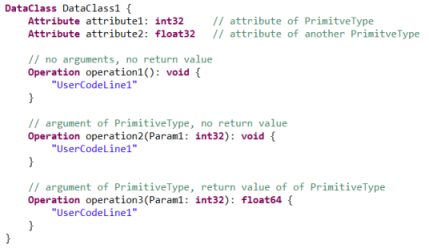
\includegraphics{images/040-DataClass1.png}
% !images/040-DataClass1.png!

Example: DataClass using other DataClasses:

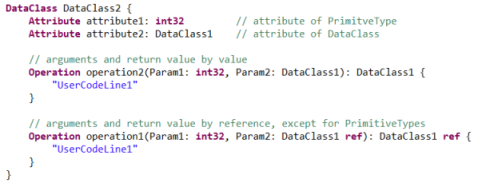
\includegraphics{images/040-DataClass2.png}
% !images/040-DataClass2.png!

\section{Layering}

\subsection{Description}

In addition to the Actor containment hierarchies, Layering provides another method to hierarchically structure a software system. Layering and actor hierarchies with port to port connections can be mixed on every level of granularity.
\begin{enumerate}
\item an ActorClass can define a Service Provision Point (SPP) to publish a specific service, defined by a ProtocolClass
\item an ActorClass can define a Service Access Point (SAP) if it needs a service, defined by a ProtocolClass
\item for a given Actor hierarchy, a LayerConnection defines which SAP will be satisfied by (connected to) which SPP
\end{enumerate}

\subsection{Notation}

\begin{table}
\begin{tabular}{|c|c|c|}
\hline
 \textbf{Description} & \textbf{Graphical Notation} & \textbf{Textual Notation} \\ \hline
 The Layer Connections in this model define which services are provided by the \textit{ServiceLayer} (\textit{digitalIO} and \textit{timer}) & 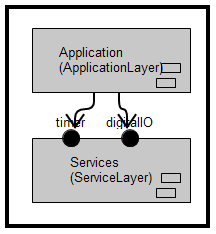
\includegraphics{images/040-LayeringModel.png} & 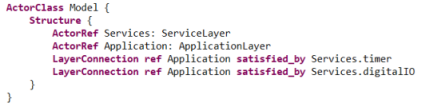
\includegraphics{images/040-LayeringModelTextual.png}  \\ \hline
 The implementation of the services (SPPs) can be delegated to sub actors. In this case the actor \textit{ServiceLayer} relays (delegates) the implementation services \textit{digitalIO} and \textit{timer} to sub actors & 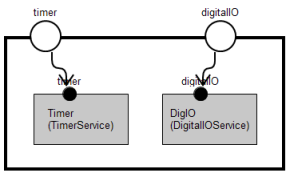
\includegraphics{images/040-LayeringServiceLayer.png} & 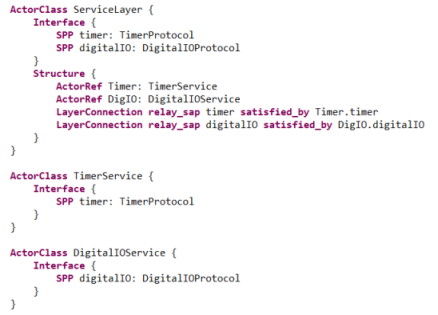
\includegraphics{images/040-LayeringServiceLayerTextual.png} \\ \hline
 Every Actor inside the \textit{ApplicationLayer} that contains an SAP with the same Protocol as \textit{timer} or \textit{digitalIO} will be connected to the specified SPP & 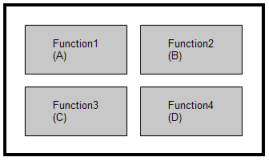
\includegraphics{images/040-LayeringApplicationLayer.png} & 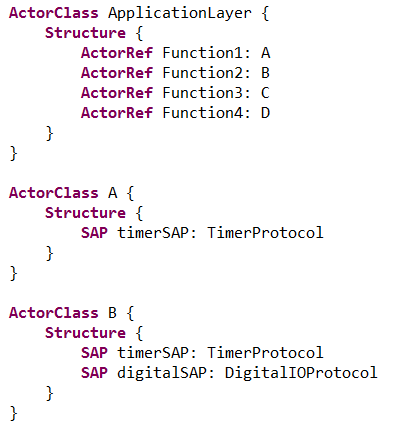
\includegraphics{images/040-LayeringApplicationLayerTextual.png} \\ \hline
\end{tabular}
\end{table}

% <table title="Title" frame="box" border="2" cellpadding="3" cellspacing="0">
	% <tr>
		% <td align="center">*Description*</td>
		% <td align="center">*Graphical Notation*</td>
		% <td align="center">*Textual Notation*</td>
	% </tr>
	% <tr>
		% <td>The Layer Connections in this model define which services are provided by the _ServiceLayer_  (_digitalIO_ and _timer_)</td>
		% <td>!images/040-LayeringModel.png!</td>
		% <td>!images/040-LayeringModelTextual.png!</td>
	% </tr>
	% <tr>
		% <td>The implementation of the services (SPPs) can be delegated to sub actors. In this case the actor _ServiceLayer_ relays (delegates) the implementation services _digitalIO_ and _timer_ to sub actors</td>
		% <td>!images/040-LayeringServiceLayer.png!</td>
		% <td>!images/040-LayeringServiceLayerTextual.png!</td>
	% </tr>
	% <tr>
		% <td>Every Actor inside the _ApplicationLayer_ that contains an SAP with the same Protocol as _timer_ or _digitalIO_ will be connected to the specified SPP</td>
		% <td>!images/040-LayeringApplicationLayer.png!</td>
		% <td>!images/040-LayeringApplicationLayerTextual.png!</td>
	% </tr>
% </table>

\section{Finite State Machines}

\subsection{Description}

Definition from "Wikipedia":http://en.wikipedia.org/wiki/Finite-state\_machine:

\begin{verbatim}
A finite-state machine (FSM) or finite-state automaton (plural: automata), or simply a state machine, is a mathematical model used to design computer programs and digital logic circuits. It is conceived as an abstract machine that can be in one of a finite number of states. The machine is in only one state at a time; the state it is in at any given time is called the current state. It can change from one state to another when initiated by a triggering event or condition, this is called a transition. A particular FSM is defined by a list of the possible states it can transition to from each state, and the triggering condition for each transition.

In ROOM each actor class can implement its behavior using a state machine. Events occurring at the end ports of an actor will be forwarded to and processed by the state machine. Events possibly trigger state transitions.
\end{verbatim}

\subsection{Motivation}

For event driven systems a finite state machine is ideal for processing the stream of events. Typically during processing new events are produced which are sent to peer actors.

We distinguish flat and hierarchical state machines.

\subsection{Notation}

\subsubsection{Flat Finite State Machine}

The simpler flat finite state machines are composed of the following elements:

\begin{table}
\caption{Title}
\begin{tabular}{|c|c|c|}
\hline
 \textbf{Description} & \textbf{Graphical Notation} & \textbf{Textual Notation} \\ \hline
 State & 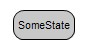
\includegraphics{images/040-State.jpg} & 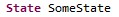
\includegraphics{images/040-StateTextual.jpg} \\ \hline
 InitialPoint & 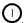
\includegraphics{images/040-InitialPoint.jpg} & \textit{implicit} \\ \hline
 TransitionPoint & 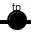
\includegraphics{images/040-TransitionPoint.jpg} & 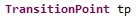
\includegraphics{images/040-TransitionPointTextual.jpg} \\ \hline
 ChoicePoint & 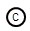
\includegraphics{images/040-ChoicePoint.jpg} & 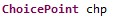
\includegraphics{images/040-ChoicePointTextual.jpg} \\ \hline
 Initial Transition & 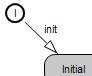
\includegraphics{images/040-InitialTransition.jpg} & 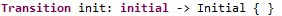
\includegraphics{images/040-InitialTransitionTextual.jpg} \\ \hline
 Triggered Transition & 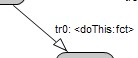
\includegraphics{images/040-TriggeredTransition.jpg} & 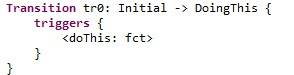
\includegraphics{images/040-TriggeredTransitionTextual.jpg} \\ \hline
\end{tabular}
\end{table}
% <table title="Title" frame="box" border="2" cellpadding="3" cellspacing="0">
	% <tr>
		% <td align="center">*Description*</td>
		% <td align="center">*Graphical Notation*</td>
		% <td align="center">*Textual Notation*</td>
	% </tr>
	% <tr>
		% <td>State</td>
		% <td>!images/040-State.jpg!</td>
		% <td>!images/040-StateTextual.jpg!</td>
	% </tr>
	% <tr>
		% <td>InitialPoint</td>
		% <td>!images/040-InitialPoint.jpg!</td>
		% <td>_implicit_</td>
	% </tr>
	% <tr>
		% <td>TransitionPoint</td>
		% <td>!images/040-TransitionPoint.jpg!</td>
		% <td>!images/040-TransitionPointTextual.jpg!</td>
	% </tr>
	% <tr>
		% <td>ChoicePoint</td>
		% <td>!images/040-ChoicePoint.jpg!</td>
		% <td>!images/040-ChoicePointTextual.jpg!</td>
	% </tr>
	% <tr>
		% <td>Initial Transition</td>
		% <td>!images/040-InitialTransition.jpg!</td>
		% <td>!images/040-InitialTransitionTextual.jpg!</td>
	% </tr>
	% <tr>
		% <td>Triggered Transition</td>
		% <td>!images/040-TriggeredTransition.jpg!</td>
		% <td>!images/040-TriggeredTransitionTextual.jpg!</td>
	% </tr>
% </table>


\subsubsection{Hierarchical Finite State Machine}

The hierarchical finite state machine adds the notion of a sub state machine nested in a state.
A few modeling elements are added to the set listed above:

\begin{table}
\caption{Title}
\begin{tabular}{|c|c|c|}
\hline
 \textbf{Description} & \textbf{Graphical Notation} & \textbf{Textual Notation} \\ \hline
 State with sub state machine &  & 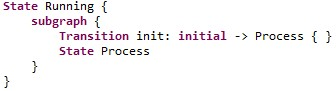
\includegraphics{images/040-StateWithSubFSMTextual.jpg} \\ \hline
 Entry Point & & 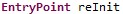
\includegraphics{images/040-EntryPointTextual.jpg} \\ \hline
 Exit Point & & 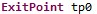
\includegraphics{images/040-ExitPointTextual.jpg} \\ \hline
\end{tabular}
\end{table}

% <table title="Title" frame="box" border="2" cellpadding="3" cellspacing="0">
	% <tr>
		% <td align="center">*Description*</td>
		% <td align="center">*Graphical Notation*</td>
		% <td align="center">*Textual Notation*</td>
	% </tr>
	% <tr>
		% <td>State with sub state machine</td>
		% <td>Parent State
		% !images/040-StateWithSubFSM.jpg!
		% Sub state machine
		% !images/040-SubFSM.jpg!</td>
		% <td>!images/040-StateWithSubFSMTextual.jpg!</td>
	% </tr>
	% <tr>
		% <td>Entry Point</td>
		% <td>In sub state machine
		% !images/040-EntryPoint.jpg!
		% On parent state
		% !images/040-EntryPointRef.jpg!</td>
		% <td>!images/040-EntryPointTextual.jpg!</td>
	% </tr>
	% <tr>
		% <td>Exit Point</td>
		% <td>In sub state machine
		% !images/040-ExitPoint.jpg!
		% On parent state
		% !images/040-ExitPointRef.jpg!</td>
		% <td>!images/040-ExitPointTextual.jpg!</td>
	% </tr>
% </table>


\subsection{Examples}

\subsubsection{Example of a flat finite state machine:}

% !images/040-FlatFSM.jpg!
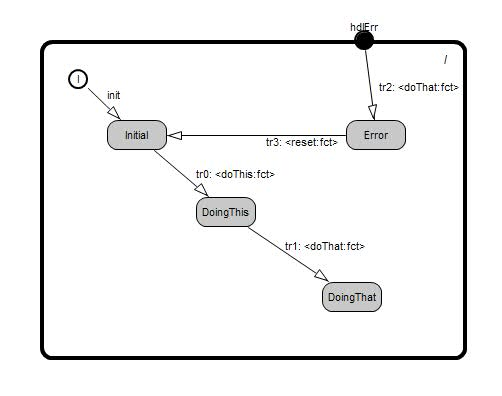
\includegraphics{images/040-FlatFSM.jpg}

\subsubsection{Example of a hierarchical finite state machine:}

Top level
% !images/040-HierarchicalFSMTop.jpg!
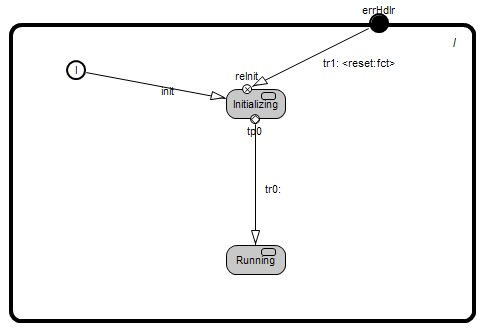
\includegraphics{images/040-HierarchicalFSMTop.jpg}

Sub state machine of Initializing
% !images/040-HierarchicalFSMInitializing.jpg!
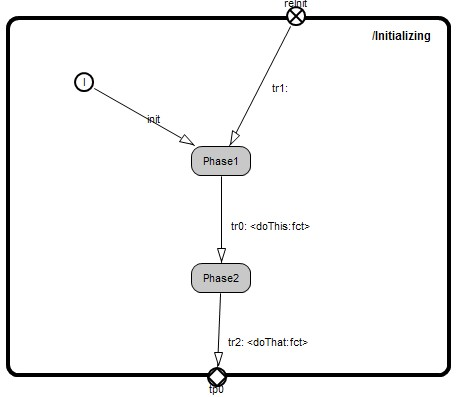
\includegraphics{images/040-HierarchicalFSMInitializing.jpg}

Sub state machine of Running
% !images/040-HierarchicalFSMRunning.jpg!
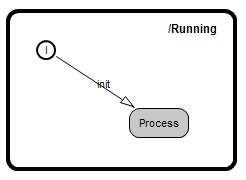
\includegraphics{images/040-HierarchicalFSMRunning.jpg}